\section{Pujoskaavio}
Solmuja voi pujoa peräkkäin useita ja monimutkaisilla tavoilla, jolloin solmujen piirtäminen käy nopeasti hyvin vaikeaksi. Monimutkaisten linkkien kuvaamiseen hyödyllinen työkalu ovat pujoskaaviot, jotka ovat tietynlaisia verkkoja. Verkko on matemaattinen olio, joka koostuu silmuista ja niitä yhdistävistä kaarista. Pujoskaavioissa kaariin liitetään kokonaislukukertoimet, jotka kertovat tietoa solmusta.

Pujoskaavioihin liittyy monta hankalaa ideaa, koska monimutkaisten linkkien esittäminen yksinkertaisesti, mutta yksiselitteisesti, on hyvin vaikeaa. Sen takia tässä kappaleessa pujoskaavioiden rakentamisessa joustetaan matemaattisesta formalismista ja lukijaa kuljetetaan eteenpäin intuitivistisesti.

Tämän kappaleen perimmäinen tarkoitus on palvella lukijaa vakuutuksena siitä, että monimutkaisten linkkien kohdalla on parempi unohtaa linkki, ja tyytyä pujoskaavioon, ja luottaa siihen, että olennaista tietoa ei menetetä.

\subsection{Pujoskaavion synty}
\label{kpl:pujoskaavion-synty}
Kappaleen 5 pujoksen määritelmän, torussolmujen ja lauseen~\ref{lause:s3-kuidutus} samankaltaisuus on tarkoituksellista. Pujoskaavion ydinajatus on, että (torus)solmun sijasta ajatellaan avaruuden, johon solmu on upotettu, rakennetta. ``Avaruuden $X$ rakenteella'' tarkoitetaan  kuidutusta $\pi:X\to Y$, joka kertoo, millä tavoin avaruuden koordinaattiakselit ``käyristyvät''. Solmu $\solmu\hookrightarrow X$ puolestaan on jokin kuitu, jonka kuva $\pi(\solmu)=y\in Y$ on yksittäinen piste.

Tällöin pujoskaaviossa riittää antaa informaatiota pelkästään avaruuden erityiskuiduista, sillä nämä määrittävät säännöllisten kuitujen rakenteen. Tämä konstruktio on intuitionvastaisuudestaan huolimatta erittäin kätevä. Syy on se, että monistojen teoria on vakiintunutta ja saatavilla oleva työkalupakki on laaja. Tämän ansiosta esimerkiksi torussolmun kaapeloiminen iteroiduksi torussolmuksi voidaan esittää \emph{monistojen kirurgian} avulla.

Monistojen kirurgia on kokoelma erilaisia tekniikoita, joilla äärellisulotteisen moniston voi muuttaa toiseksi $M\leadsto N$, vaikka $M$ ja $N$ eivät olisi keskenään diffeomorfisia. Yksinkertaisin esimerkki kirurgiasta on lauseen~\ref{lause:s3-kuidutus} topologisen todistuksen konstruktio $\S^2\times\S^1\leadsto\S^3$. Konstruktiossa monistosta $\S^2\times\S^1$ ``porattiin'' kaksi torusta pois, mistä jääneet aukot ``täytettiin'' vääntyneillä toruksilla.

Määritellään pujoskaavio konstruktion kautta, jonka jälkeen annetaan yksinkertaisia esimerkkejä.
\begin{konstruktio}
    \label{konstruktio:pujoskaavio}
    Kuvassa~\ref{kuva:torussolmuja-eri-tavoin} on esitetty torussolmut $(2,3)$ ja $(2,7)$ kolmella eri tavalla. Vasemmalta oikealle nämä ovat tavallinen solmuesitys, homologia-akseleittain ja pujoskaaviolla.
    \begin{figure*}
        \centering
        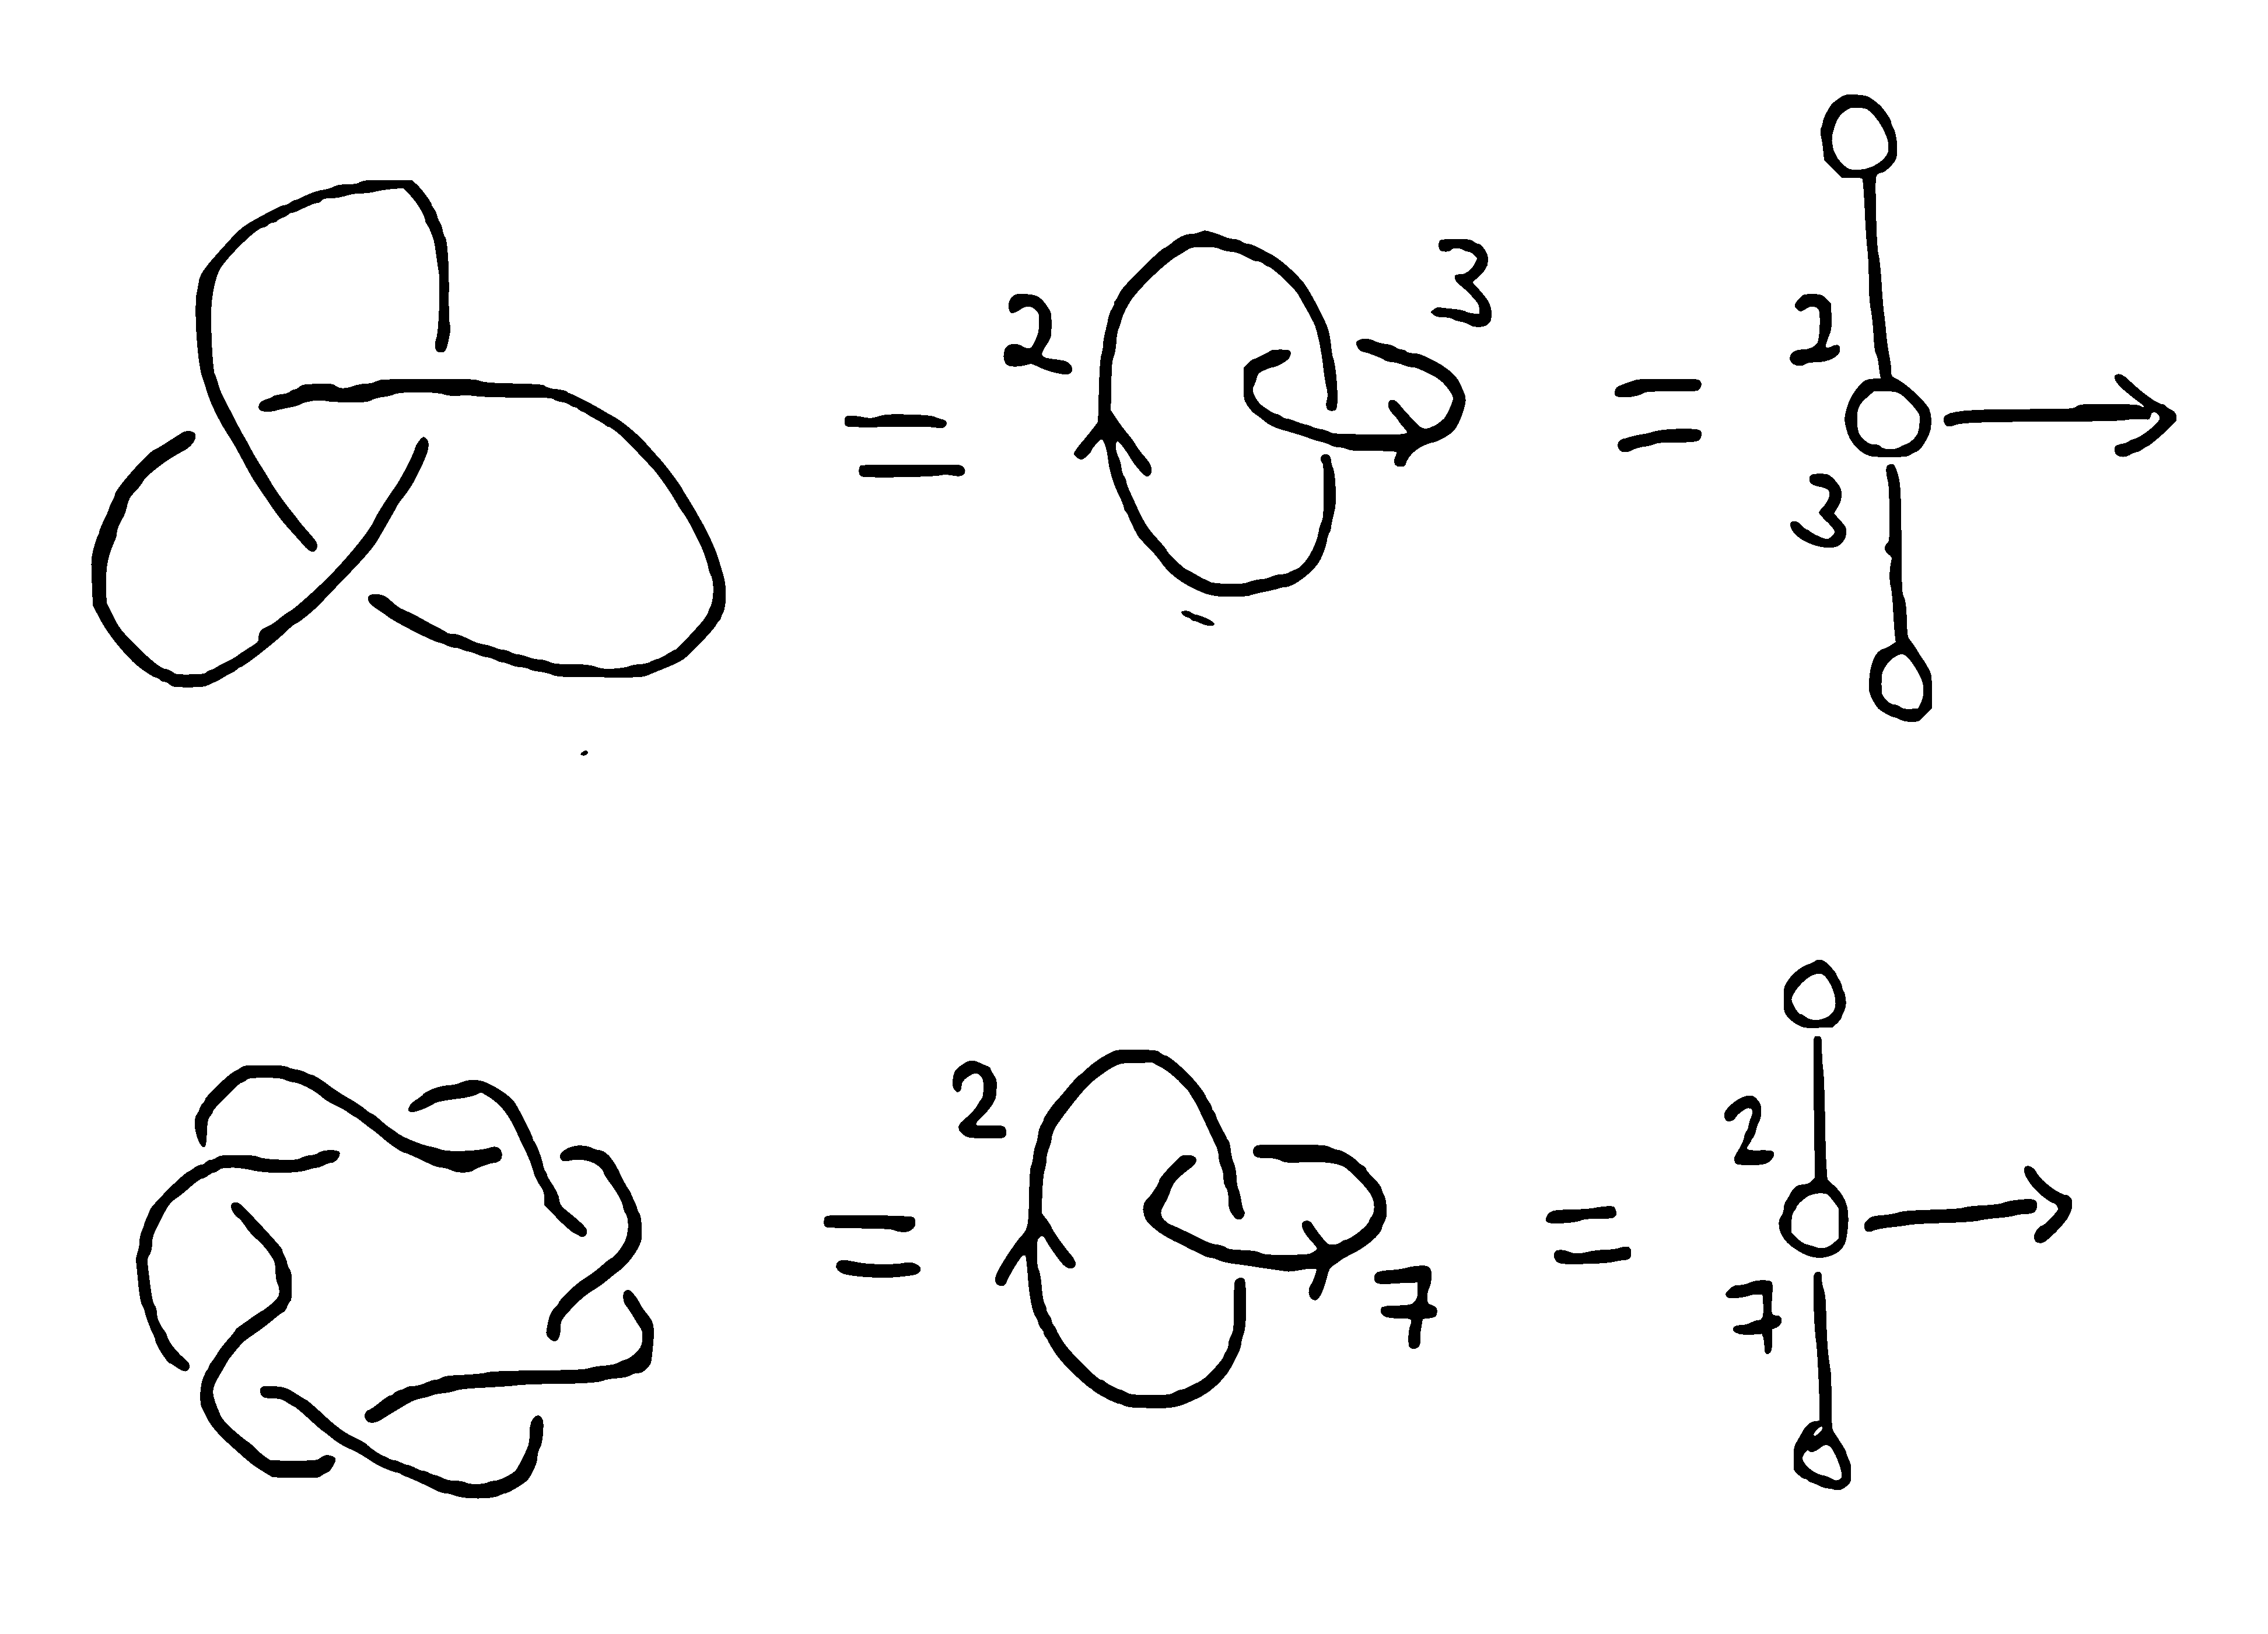
\includegraphics[width=0.5\textwidth]{figures/torussolmuja-homologia-akseleita-ja-pujoskaavioita.pdf}
        \caption{Kaksi torussolmua eri tavoin esitettyinä.}
        \label{kuva:torussolmuja-eri-tavoin}
    \end{figure*}
    Pujoskaaviossa on kolmenlaisia komponentteja, jotka on piirretty alle.
    \begin{center}
        \begin{tikzpicture}
            % --- CRÉATION DES NŒUDS ---
            % Vous positionnez vos nœuds de base ici.
            % On place le symbole \Gamma entre les accolades à la fin
            % \node[rectangle node] (Gamma) at (0,0) {$\Gamma$};
            \node[solid node] (A) at (0,0) {};
            \node[empty node] (B) at (1.5,0) {};
            \node[placeholder] (a) at (1,0) {};
            \node[placeholder] (b) at (2.5,0) {};
            \node[placeholder] (c) at (3,0) {};

            % --- 2 & 5) FLÈCHES VERS LE VIDE ---
            % LaTeX ne peut pas deviner l'espace vide absolu sans direction.
            % La syntaxe "++(angle:distance)" est idéale : vous donnez juste un angle 
            % (ex: 135 degrés) et une longueur (ex: 1cm), et LaTeX calcule 
            % automatiquement la coordonnée finale dans l'espace vide.
            \draw[->, thin] (c) -- ++(0:1cm);

            % --- 3) ARÊTES AVEC VALEURS AUX DEUX EXTRÉMITÉS ---
            % "near start" et "near end" placent les entiers automatiquement aux bouts.
            % L'option "swap" [xxx, yyy, swap] (ou ') permet de basculer le texte de l'autre côté de la ligne.
            \draw (A) -- node[edge value, near start] {$\alpha$}
                        node[edge value, near end] {} (a);
                        
            \draw (B) -- node[edge value, near start] {$\beta$} 
                        node[edge value, near end] {} (b);

        \end{tikzpicture}
    \end{center}
    Tässä $\alpha,\beta$ ovat joitain kokonaislukuja. Merkitään komponentteja tekstin seassa $\bullet,\circ,\rightarrow$. Joissakin tilanteissa on hyödyllistä \emph{juurtaa} kaavio, eli valita mielivaltaisesti jokin silmuista kaavion juureksi. Juurta merkitään $\bullet$. Juurtamaton kaavio sisältää vain tyypillisiä silmuja $\circ$ ja nuolia $\rightarrow$.

    Palloa $\circ$ (tai $\bullet$) käytetään kuvaamaan avaruutta, jossa linkki elää. Jos $\linkki=(\Sigma,\solmu_1)$, niin $\circ$ on $\Sigma$. Tässä työssä $\Sigma$ on aina $\S^3$. Lauseen~\ref{lause:s3-kuidutus} nojalla $\S^3$ voidaan kuiduttaa jollakin epätriviaalilla tavalla. Tämän vuoksi on tarpeellista esittää pallon $\circ$ yhteydessä myös tietoa kuidutuksesta. Jos $k_1,k_2$ ovat kuidutuksen määräävät kokonaisluvut, ts. erityiskuitujen moninkerrat, ilmaistaan tämä pujoskaaviolla
    \begin{center}
        \begin{tikzpicture}
            \node[empty node] (A) at (0,0) {};
            \node[empty node] (k1) at (0,1) {};
            \node[empty node] (k2) at (0,-1) {};

            \draw (A) -- node[edge value, near start] {$k_1$}
                         node[edge value, near end] {} (k1);
            \draw (A) -- node[edge value, near start, swap] {$k_2$}
                         node[edge value, near end] {} (k2);
        \end{tikzpicture}
    \end{center}
    Pallot $\circ$ voikin itse asiassa jakaa kahteen luokkaan: \emph{lehdiksi}, joilla on vain yksi kaari ja \emph{silmuiksi}, joilla voi olla useampi kaari. Silmu symboloi avaruutta $\S^3$ ja lehteä puolestaan avaruuden erityiskuitua. Lehden kaarelle voidaan asettaa kokonaisluku, joka kertoo kyseisen erityiskuidun kertaluvun.

    Teknisesti ottaen triviaalisti kuidutetun avaruuden pujoskaavioon voitaisiin piirtää lehdet siten, että $k_1=k_2=1$, mutta on mielekästä piirtää kaavioista mahdollisimman minimaalisia. Jos $k_2=1$, mutta $k_1>1$, niin avaruudella on vain yksi erituiskuitu, jolloin säännölliset kuidut eivät homologisesti poikkea triviaalista tapauksesta.

    Nuolet $\rightarrow$ vastaavat linkin komponentteja. Nuoli $\rightarrow$ on \emph{aina} kiinnitetty silmuun $\circ$ tai $\bullet$ ja se tarkoittaa jotakin yhtä (mielivaltaista) kuitua avaruudessa, johon se on kiinnitetty. Nuoli voi kuvata säännöllistä kuitua, jolloin sille ei tarvitse antaa kokonaislukua, tai erityiskuitua jolloin sille annetaan kokonaisluku samaan tapaan kuin lehdillekin. On tosin huomattava, että $\S^3$:lla voi olla korkeintaan kaksi erityiskuitua.

    Yksinkertaisin solmu, epäsolmu $\bigcirc\hookrightarrow\S^3$ voidaan esittää kaaviolla
    \begin{center}
        \begin{tikzpicture}
            \node[empty node] (A) at (0,0) {};
            \draw[->, thin] (A) -- ++(0:1cm);
        \end{tikzpicture},
    \end{center}
    jossa $\circ$ vastaa 3-palloa ja $\rightarrow$ siihen upotettua epäsolmua. Jos $\linkki=(\S^3,\solmu_1\cup\cdots\cup\solmu_n)$ ja $\linkki'=(\S^3,\solmu_{n+1}\cup\cdots\cup\solmu_m)$ ovat linkkejä, niin näiden linkkien pujos komponentteja $\solmu_i\in\linkki,\solmu_j\in\linkki'$ myöden voidaan kuvata kaaviolla
    \begin{center}
        \begin{tikzpicture}
            \node[rectangle node] (L1) at (0,0) {$\linkki$};
            \node[text box] (plus) at (1.5,0) {$+$};
            \node[rectangle node] (L2) at (3,0) {$\linkki'$};
            \node[text box] (equals) at (4,0) {$=$};
            \node[rectangle node] (l1) at (5,0) {$\linkki$};
            \node[rectangle node] (l2) at (7,0) {$\linkki'$};

            \draw[->] (L1) -- ++(0:1cm);
            \draw[->] (L2) -- ++(180:1cm);

            \draw (l1) -- node[edge value, near start] {}
                          node[edge value, near end] {} (l2);
        \end{tikzpicture}
    \end{center}
    ja linkeille $\linkki,\linkki'$ voi muodostaa induktiivisesti samoja periaatteita noudattaen omat kaavionsa. Tällaista kaaviota kutsutaan \emph{pujoskaavioksi.}
\end{konstruktio}
\begin{maaritelma}[Pujoskaavio]
    Kutsutaan konstruktiossa~\ref{konstruktio:pujoskaavio} esiteltyjä puuverkkoja \emph{pujoskaavioiksi} ja puuverkkojen erilaisia komponentteja \emph{lehdiksi}, \emph{silmuiksi}, \emph{nuoliksi}, \emph{kaariksi} ja \emph{juuriksi} siten kuin konstruktiossa on kyseisiä sanoja konstruktiossa käytetty.

    Olkoon $\linkki=(\S^3,\solmu_1\cup\cdots\solmu_n)$ linkki. Merkitään linkin pujoskaaviota $\Gamma(\linkki)=\Gamma(m)=\Gamma(m_1,\dots,m_n)$, jossa $m_i$ on solmun $\S_i$ kertaluku. Kertaluvun $m_i$ positiivisuus tai negatiivisuus kertoo solmun suunnistuksen.

    Vastaavasti jos $\Gamma$ on pujoskaavio, olkoon $\linkki(\Gamma)$ kaaviota vastaava linkki.
\end{maaritelma}
\begin{huomautus}
    Annetussa pujoskaavion konstruktiossa ainoa keino välittää informaatiota avaruuksien tai käyrien suunnistuksesta on kuituja kuvaavien kokonaislukujen positiivisuus tai negatiivisuus. Täyden tarkkuuden saavuttamiseksi kaavion pitäisi välittää tietoa myös pohja-avaruuden suunnistuksesta. Lauseessa~\ref{lause:pujoskaaviopläjäys} kuitenkin osoitetaan, että käytännössä avaruuksien voi aina olettaa olevan positiivisesti suunnistettuja.
\end{huomautus}
Kun pujoskaaviot on nyt esitelty, tutkitaan joitakin esimerkkejä.

% Epäsolmujen erillinen solmu
\begin{esimerkki}[Erillinen summa]
    Kahden epäsolmun (tai yleisemmin linkin) erillistä summaa kuvataan erillisillä pujoskaavioilla
    \begin{center}
        \begin{tikzpicture}
            \node[empty node] (A) at (0,0) {};
            \node[empty node] (B) at (1.5,0) {};

            \draw[->] (A) -- ++(0:1cm);
            \draw[->] (B) -- ++(0:1cm);
        \end{tikzpicture}
    \end{center}
\end{esimerkki}
% Kahden epäsolmun pujominen
\begin{esimerkki}
    Esimerkiksi jos kaksi epäsolmua $(\S^3,\solmu_1),(\S^3,\solmu_2)$ pujotaan yhteen, on tuloksena tyhjä $\S^3$ ilman yhtäkään solmua, kuten lemma~\ref{lemma:s3-torushajotus} osoittaa.
    \begin{center}
        \begin{tikzpicture}
            \node[empty node] (A) at (0,0) {};
            \node[text box] (plus) at (1.5,0) {$+$};
            \node[empty node] (B) at (3,0) {};
            \node[text box] (equals1) at (4,0) {$=$};
            \node[empty node] (a) at (5,0) {};
            \node[empty node] (b) at (6.5,0) {};
            \node[text box] (equals2) at (4,-0.75) {$=$};
            \node[empty node] (ab) at (5,-0.75) {};

            \draw[->] (A) -- ++(0:1cm);
            \draw[->] (B) -- ++(180:1cm);
            \draw (a) -- node[edge value, near start] {} 
                         node[edge value, near end] {} (b);
        \end{tikzpicture}
    \end{center}
\end{esimerkki}
Lauseen~\ref{lause:s3-kuidutus} topologisessa todistuksessa tehtiin liimausoperaatio, jossa liimattiin vääntyneitä toruksia. 
\begin{esimerkki}(Torussolmut)
    Torussolmu $\solmu(p,q)\subset\S^3$ voidaan esittää kuidutuksen $\pi_{p,q}:\S^3\to\S^2$ säännöllisenä kuituna. Siispä $(p,q)$-torussolmun pujoskaavio on
    \begin{center}
        \begin{tikzpicture}
            \node[empty node] (A) at (0,0) {};
            \node[empty node] (p) at (0,1) {};
            \node[empty node] (q) at (0,-1) {};

            \draw[->] (A) -- ++(0:1cm);

            \draw (A) -- node[edge value, near start] {$p$}
                         node[edge value, near end] {} (p);
            \draw (A) -- node[edge value, near start, swap] {$q$}
                         node[edge value, near end] {} (q);
        \end{tikzpicture}
    \end{center}
\end{esimerkki}
% S(p,q)=S(q,p) pujoskaavioilla
\begin{esimerkki}
    Lemma~\ref{lemma:pq-torussolmu-on-qp} saa pujoskaavioiden avulla muodon
    \begin{center}
        \begin{tikzpicture}
            \node[empty node] (A) at (0,0) {};
            \node[empty node] (K1) at (0,1) {};
            \node[empty node] (K2) at (0,-1) {};
            \node[text box] (equals) at (2,0) {$=$};
            \node[empty node] (a) at (3.5,0) {};
            \node[empty node] (k1) at (3.5,-1) {};
            \node[empty node] (k2) at (3.5,1) {};

            \draw[->] (A) -- ++(0:1cm);
            \draw[->] (a) -- ++(0:1cm);

            \draw (A) -- node[edge value, near start] {$k_1$}
                         node[edge value, near end] {} (K1);
            \draw (A) -- node[edge value, near start, swap] {$k_2$}
                         node[edge value, near end] {} (K2);
            \draw (a) -- node[edge value, near start, swap] {$k_1$}
                         node[edge value, near end] {} (k1);
            \draw (a) -- node[edge value, near start] {$k_2$}
                         node[edge value, near end] {} (k2);
        \end{tikzpicture}
    \end{center}
\end{esimerkki}
\begin{esimerkki}[Iteroitu torussolmu]
    Kaapeloidaan $(p_1,q_1)$-torussolmu $\solmu$ $(p_2,q_2)$-kaapelilla. Olkoon $\S_1^3$ avaruus, jossa $\solmu$ elää ja $\T\subset\S^3$ torus, jonka pinnalle $\solmu$ voidaan piirtää. Tällöin $\solmu$ kulkee $p_1$ kertaa pituuspiirin ympäri ja $q_1$ kertaa ympäryspiirin ympäri.

    Kaapelin pujoskaavio on
    \begin{center}
        \begin{tikzpicture}
            \node[empty node] (A) at (0,0) {};
            \node[empty node] (p2) at (0,1) {};
            \node[placeholder] (q2) at (-1,0) {};
            \node[placeholder] (k) at (0,-1) {};

            \draw[->] (A) -- ++(180:1cm);
            \draw[->] (A) -- ++(-90:1cm);

            \draw (A) -- node[edge value, near start, swap] {$p_2$}
                         node[edge value, near end] {} (p2);
            \draw (A) -- node[edge value, near start] {$q_2$}
                         node[edge value, near end, swap] {} (q2);
            \draw (A) -- node[edge value, near start] {$1$}
                         node[edge value, near end] {} (k);
        \end{tikzpicture}
    \end{center}
    Kaapeli on kahden solmun linkki. Avaruudella $\S_2^3$, jossa kaapeli elää on, kuidutus $\pi_{p_2,q_2}:\S^3-\S^2$. Solmut avaruudessa ovat säännöllinen kuitu on kertaluvulla 1 (torussolmu $\solmu'=\solmu'(p_2,q_2)$) ja erityiskuitu kertaluvulla $q_2$ (epäsolmu). Jos erityiskuitu eli epäsolmu pujotaan torussolmuun $\solmu(p_1,q_1)$, liimatessa $\S_2^3\setminus\solmu'$ avaruuteen $\S_1^3\setminus\solmu$ täytyy ensimmäistä vääntää niin rajusti, että $\solmu'(p_2,q_2)$ muuttuu iteroiduksi.
    \begin{center}
        \begin{tikzpicture}
            % torussolmu
            \node[empty node] (B) at (0,0) {};
            \node[empty node] (p1) at (0,1) {};
            \node[empty node] (q1) at (0,-1) {};
            \node[placeholder] (arrow1) at (1,0) {};
            % kaapeli
            \node[empty node] (A) at (3,0) {};
            \node[empty node] (p2) at (3,1) {};
            \node[placeholder] (q2) at (2,0) {};
            \node[placeholder] (arrow2) at (3,-1) {};
            % iteroitu torussolmu
            \node[empty node] (b) at (6,0) {};
            \node[empty node] (pp1) at (6,1) {};
            \node[empty node] (qq1) at (6,-1) {};
            \node[empty node] (a) at (8,0) {};
            \node[empty node] (pp2) at (8,1) {};
            \node[placeholder] (arrow3) at (8,-1) {};
            % tekstit
            \node[text box] (plus) at (1.5,0) {$+$};
            \node[text box] (equals) at (4.5,0) {$=$};

            % torussolmu
            \draw[->] (B) -- ++(0:1cm);
            % kaapeli
            \draw[->] (A) -- ++(180:1cm);
            \draw[->] (A) -- ++(-90:1cm);
            % iteroitu torussolmu
            \draw[->] (a) -- ++(-90:1cm);

            % torussolmu
            \draw (B) -- node[edge value, near start] {$p_1$}
                         node[edge value, near end] {} (p1);
            \draw (B) -- node[edge value, near start, swap] {$q_1$}
                         node[edge value, near end] {} (q1);
            \draw (B) -- node[edge value, near start] {$1$}
                         node[edge value, near end] {} (arrow1);
            % kaapeli
            \draw (A) -- node[edge value, near start, swap] {$p_2$}
                         node[edge value, near end] {} (p2);
            \draw (A) -- node[edge value, near start, swap] {$q_2$}
                         node[edge value, near end] {} (q2);
            \draw (A) -- node[edge value, near start] {$1$}
                         node[edge value, near end] {} (arrow2);
            % iteroitu torussolmu
            \draw (b) -- node[edge value, near start] {$p_1$}
                         node[edge value, near end] {} (pp1);
            \draw (b) -- node[edge value, near start, swap] {$q_1$}
                         node[edge value, near end] {} (qq1);
            \draw (b) -- node[edge value, near start] {$1$}
                         node[edge value, near end] {$q_2$} (a);
            \draw (a) -- node[edge value, near start, swap] {$p_2$}
                         node[edge value, near end] {} (pp2);
            \draw (a) -- node[edge value, near start] {$1$}
                         node[edge value, near end] {} (arrow3);
        \end{tikzpicture}
    \end{center}
\end{esimerkki}

\subsection{Pujoskaavioiden ominaisuuksia}
Tässä kappaleessa käsitellään muodollisesti pujoskaavioiden ominaisuuksia ja todistetaan joitakin hyödyllisiä tuloksia.
\begin{propositio}
    Linkki $\linkki=(\Sigma,K)$ on kompleksitason käyrän singulariteetin linkki jos ja vain jos sillä on yhtenäinen pujoskaavio, jonka kaikki painot ja kaarideterminantit ovat positiivisia. Tällöin sillä on minimaalinen pujoskaavio näillä ominaisuuksilla.
\end{propositio}
\begin{proof}
    En tiedä.
\end{proof}
\begin{lemma}
    Kahden linkin osasen (virtuaalisen tai todellisen) linkkiluku $\Sigma$:ssa saadaan laskemalla pujoskaaviossa osasten välillä olevan polun viereisten painojen tulo.
\end{lemma}
\begin{proof}
    En tiedä.
\end{proof}

\begin{propositio}
    Polynomisolmun pujoskaavion sidoskertoimet saadaan kaavoista $\alpha_1=q_1$ ja $\alpha_{i+1}=q_{i+1}+q_i p_i p_{i+1}$, missä $p_i,q_i$ ovat polynomin Puiseux-dataa.
\end{propositio}
\begin{proof}
    \citep{EN1985}[Prop 1A.1]
\end{proof}


\subsection{Monimutkainen esimerkki}
Tässä kappaleessa tutustutaan monimutkaiseen solmuun ja sen pujoskaavion rakentamiseen sekä mielellään myös toisin päin.
